\documentclass[conference]{IEEEtran}

\ifCLASSINFOpdf
\else
\fi
\usepackage{url}
\usepackage[hypcap]{caption}
\usepackage{listings}
\usepackage{pgfplots}
\usepackage{pgfplotstable}
\usepackage{eurosym}
\usepackage{multirow}
\usepackage{subfigure}

%\usepackage{caption}
%\usepackage{subcaption}

\usetikzlibrary{backgrounds}
\pgfplotsset{compat=1.5}
\usepgfplotslibrary{dateplot}


\begin{document}
\title{A Case Study of Web API Evolution}


\author{\IEEEauthorblockN{S M Sohan, Craig Anslow, Frank Maurer
\IEEEauthorblockA{Department of Computer Science\\
University of Calgary,
Calgary, Alberta T2N 1N4\\ Email: \{smsohan, craig.anslow, frank.maurer\}@ucalgary.ca }
}}

\maketitle


\begin{abstract}
When applications are integrated using web APIs, changes on a web API may break the dependent applications. This problem exists because old versions of the APIs may no longer be supported, a lack of adequate documentation to upgrade to a newer version, and insufficient communication of changes. In this paper we conducted a case study of evolving Web APIs to investigate what changes are made between versions and how the changes are documented and communicated to the API users. The findings are a list of recommendations for practitioners and researchers based on API change profiles, versioning, documentation and communication approaches that are observed in practice. This study will help inform developers of evolving Web APIs to make decision about versioning, documentation and communication methods.
\end{abstract}


\begin{IEEEkeywords}
Case Study; RESTful, SOAP, Web API Evolution; WSDL
\end{IEEEkeywords}

\IEEEpeerreviewmaketitle

\section{Introduction}

Web APIs are used as a key interconnectivity mechanism to access software services over the Internet. Interconnected applications can provide better service at a lower cost to their users. For example, a business search portal can display the businesses near a user's current location on a map by using the Google Maps API. The actual implementation of Web APIs can follow various protocols, such as SOAP\footnote{http://www.w3.org/TR/soap/} and RESTful\footnote{\url{http://www.ics.uci.edu/~fielding/pubs/dissertation/rest_arch_style.htm}} web services. In this paper, the term Web API is used to describe any protocol unless otherwise specified.

Web APIs connect independently maintained applications. As a result, when a Web API evolves, all the integrated applications using the Web API may not be able to evolve on the same schedule. For example, in the case of the aforementioned business search portal, if the Google Maps API changes, it may also require the portal to change. This introduces unique challenges to the evolution of Web APIs compared because the evolution is out of the control of the API users. For example, API users of a local API can use a copy of an older version, but for evolving Web APIs, API users are forced to upgrade if older versions are no longer supported. Documentation of evolving Web APIs is an important topic for case study because of the unique challenges it presents. Web APIs are defined by their HTTP interface, including both HTTP headers as well as request and response data formats. As a result, for an evolving Web API, its documentation needs to indicate changes in any of these fields, unlike the local APIs, where typically no HTTP specific information is involved.

The primary goal of this research is to investigate the challenges that are currently faced by developers and users of evolving Web APIs so that future research can be performed to address the problems. To this regard, we analyzed existing literature on the topic of Web API evolution. We analyzed the evolution of multiple Web APIs to understand the current industry trends and challenges. The juxtaposition of current industry practices with the literature reveals insights that are otherwise unseen when viewed from a single perspective. We use the differences between the literature and industry practices to identify unresolved research problems.

In this case study, multiple Web APIs representing a variety of application areas are selected, analyzed and compared to gain a broader perspective about current industry practices on Web API versioning, documentation and communication of changes. The result of this analysis is a summary of different approaches to Web API evolution, and a list of recommendations for developers of evolving Web APIs.

The remainder of this paper is organized as follows: the next section is related work on Web API evolution. Then, we discuss the case study of multiple Web API evolution. In the following section, we list our findings, followed by a discussion about the findings. Finally, we conclude with the contributions of this work.

\section{Related Work}

We look at related work in the following areas: Empirical Research on Web API evolution, techniques to evolve Web APIs and, tool support for evolving Web APIs.

\subsection{Empirical Research on Web API evolution} % (fold)
\label{sub:empirical_research}
Several case study papers were published on Web API Evolution. Maleshkova et al. analyzed multiple Web APIs to identify the different approaches related to Web API descriptions, data formats, protocols, reusability, granularity, and authentication \cite{maleshkova}. They found that a lack of a standard format to document Web APIs and manual documentation led to API under-specification causing confusions about how to use the APIs for different use cases. They identified a need for automated approaches.

Fokaefs et al. performed an empirical study on Web API evolution involving multiple SOAP web services, Amazon EC2, FedEx Rate, Bing, Paypal, and Fedex Pack., and provided an evolution profile showing the percentage of changes between two consecutive versions of the Web APIs \cite{fokaefs_2011_empirical}. The same Web APIs were studied by Romano et at., but they provided an alternate evolution profile of the Web APIs. Instead of using percentage of change, they profiled the number of operations, parts and XML file elements from WSDL files for each version of the Web APIs \cite{wsdl_diff_2012}. These change profiles point to the ever changing nature of Web APIs.

Jun et al. performed case studies on the evolution of Web APIs and compared the evolution of Web APIs against local library APIs \cite{li_client_2013}. For studying Web APIs, a selection criteria was provided as follows: Web APIs with large number of clients, covering different application areas, owned by different companies in different countries, and well documented API reference and migration guides. They extracted 16 patterns to describe different types of changes on the Web APIs as follows: add or remove parameter, change type of return value, delete method, rename method, rename parameter, change format of parameter, change format of return value, change XML tag, combine methods, split method, expose data, unsupport request method, change default value of parameter, chance default value of parameter, change upper bound of parameter, restrict access to API. They also presented six challenges specific to Web API evolution that are not found with library APIs such as: transformation between JSON and XML, M to N Mapping, delete method, authorization protocol change, rate limit, and authorization of API access.

Espinha et al. looked at the growing pains with Web API evolution from the perspective of Web API users by conducting interviews \cite{espinha}. The interviewees were selected based on the activity of their open-source projects that used Web APIs. They found that when a Web API evolves, maintaining the integration with a Web API took more effort than integrating it the first time since maintenance is carried out over a longer period of time. This makes the evolution of Web APIs an important subject for a case study.

We distinguish our case study from these case studies as follows: we provide up-to-date information and include a diverse set of Web APIs. Our analysis uses new data sources such as API user forums, and question and answer sites. We focused this study on different approaches to versioning, documentation, and communicating changes as an API evolves.
% subsection empirical_research (end)

\subsection{Techniques to evolve Web APIs} % (fold)
\label{sub:techniques}
Kaminski et al. presented a design technique called ``Chain of Adapters'' to implement evolving Web APIs \cite{kaminski2006design}. Using this approach, the source code of a Web API can evolve from a version to the next by introducing an adapter on the original version to implement any required change for new versions. This technique allows for multiple versions to be deployed concurrently since older versions are left unchanged.

Leskey suggests following a consistent and meaningful naming scheme to identify different versions of APIs \cite{laskey2008considerations}. Such a naming scheme can be used to identify if two versions of an API are compatible. Given the URL scheme, Leskey suggests a self documenting Web API, one that exposes API endpoints to describe the details for each version.

Treiber et al. showed a conceptual model to capture the changes of a Web API \cite{treiber2009analyzing}. A graphical representation to display the evolution of SOAP Web Services is presented by Aversano et al. where the differences between versions are highlighted based on their meta information found in the WSDL files \cite{aversano2005visualizing}.

Some papers focused on automatic migration of Web API clients to newer versions. For example, Wilde proposed a conceptual framework where WSDL can be extended so a client can be compatible with potential Web API changes \cite{wilde2004semantically}. A similar approach is proposed by Fang et al. where a fixed set of new XML nodes are used instead of arbitrary extensions \cite{fang2007version}. Juric et al. proposed a number of versioning related extensions to WSDL that can be applied to version SOAP web services in multiple levels of granularity such as, service level and operation level \cite{Juric20091326}. Zuo et al. developed a formal XML based change specification format to describe the evolution of SOAP Web services \cite{zuo6928972}.

For RESTful Web APIs, Mangler et al. introduced an XML based language called RIDDL \cite{mangler2010origin}. RIDDL allows incremental composition of Web API documentation for different versions by adding a changelog to the documentation of an old version.

VRESCo demonstrates an approach where a router between the Web API client and server is used to automatically route Web API calls to new API versions. The router routes API calls to the desired version based on free form version names such as: latest, stable, and fixed version \cite{leitner2008end}. Meng et al. compared different approaches for evolving Web APIs across multiple criteria: granularity of evolution, terminal of evolution, type of evolution, scalability, and maintainability \cite{6835564}. They identified an aspect oriented approach, where an intermediate tier between a Web API and its clients is used similar to VRESCo, can reduce coupling between the two.

Existing techniques to evolve Web APIs focused on finding different techniques for implementing evolving SOAP based Web APIs that cannot be readily applied to RESTful Web APIs. From our case study, we identified future research opportunities on techniques to solve the problems Web API evolution that are also applicable to RESTful APIs.

\subsection{Tool support for evolving Web APIs} % (fold)
\label{sub:tool_development}

%{|p{0.2\linewidth}|p{0.3\linewidth}|p{0.2\line width}|p{0.2\linewidth}|}
%& &  \multicolumn{4}{ c |}{\textbf{Categories}} & & \\ \cline{3-6}
%\multirow{2}{*}{\textbf{Web API}}  & \multirow{2}{*}{\textbf{URL}} &\textbf{Industry} & \textbf{Popularity} &  \textbf{Maturity} & \textbf{Code}& \multirow{2}{*}{\\textbf{Rel.}} & \multirow{2}{*}{\\textbf{Dates}}\\

\begin{table*}[!ht]
\caption{Case Study - Representative Sample of Web APIs.}
\label{web_api_grid}
\begin{tabular} {| l | l  | l  | l | l | l | l  | l |}
\hline
\multirow{2}{*}{\textbf{Web API}} &
\multirow{2}{*}{\textbf{URL}} &
\multicolumn{4}{ c |}{\textbf{Categories}} &
\textbf{Num of} &
\multirow{2}{*}{\textbf{Dates}}\\    \cline{3-6}
  & & Industry & Popularity &  Maturity & Code& \textbf{Releases}& \\
\hline
Facebook Platform API & \tiny{\url{https://developers.facebook.com/docs/apps/versions}} & Social & High & Est & Closed & 11 & 01/2013-07/2014\\
\hline
Twitter REST API & \tiny{\url{https://dev.twitter.com/docs/api}} & Social & High & Est & Closed & 2 & Not Available\\
\hline
Wordpress REST API & \tiny{\url{http://wp-api.org/}} & Business & Growing &  New & Open & 8 & 08/2013-06/2014\\
\hline
Salesforce \& Chatter REST API & \tiny{\url{https://www.salesforce.com/us/developer/docs/api_rest/}} & Business & Popular & Est & Closed & 4 & 01/2013-08/2014\\
\hline
Google Calendar API & \tiny{\url{https://developers.google.com/google-apps/calendar/}} & Business & Popular & Est & Closed & 2 & Not Available\\
\hline
Stripe Payment Processor API & \tiny{\url{https://stripe.com/docs/api}} & Business & Growing & New & Closed & 30 &09/2011-10/2014 \\
\hline
Github API & \tiny{\url{https://developer.github.com/}} & Productivity & Growing & New & Closed  & 59 &09/2012-10/2014\\
\hline
Google Maps API & \tiny{\url{https://developers.google.com/maps/web/}} & Productivity & Popular & Est & Closed & 102 &01/2011-09/2014\\
\hline
OpenStreetMap API &\tiny{\url{http://wiki.openstreetmap.org/wiki/API}} & Productivity & Growing & New & Open & 1 & Not Available\\
\hline
\end{tabular}
\end{table*}

Analyzing the available tool support for evolving Web APIs helped us identify opportunities for future research in this area. WSDarwin introduces a layer of adapters on both the Web API and its client to automatically migrate Web API clients to use a newer version of an API \cite{WSDarwin}. WSDarwin uses WSDL description of the SOAP service to automatically infer the changes between versions and uses preset default values for newly added objects to adapt the client request. VTracker, predecessor of WSDarwin, produces a changelog between versions of WSDL files \cite{fokaefs_2011_empirical}. WSDLDiff extends this by incorporating the semantic meaning of WSDL with an XML Schema Definition into their changelog computation \cite{wsdl_diff_2012}.

To identify if a new version of a Web API has any impact on a specific API client,  Zou et al. show a technique to generate client specific change logs \cite{le2008synchronizing}. A customized per API client change log is generated by filtering the change log based on  recorded API usage data so that only relevant API changes can be communicated effectively to each user.

Existing research on tool support for RESTful Web API evolution is rather limited. hRESTS is an HTML-based specification for describing RESTful Web APIs that can be used by computers to auto-generate client code \cite{4740521}. RESTdesc is another specification for describing RESTful Web API documentation where APIs are described using pre and post conditions \cite{RESTdesc}. However, the input to both hRESTS and RESTDesc require manual effort to produce the desired specification.

In the literature, we found multiple tools exist that rely on WSDL files. WSDL solutions have limited applicability for RESTful Web APIs since WSDL files cannot be used to fully describe RESTful APIs. Based on our case study, we will discuss future research problems on tool development to support the challenges with RESTful Web API evolution.

\section{Case Study}
When companies evolve their Web APIs in practice the new changes can often break applications that rely on these APIs. The aim of this case study is to investigate current industry practices on Web API Evolution to answer the following research questions.

\subsection{Research Questions} % (fold)

\begin{description}
  \item[RQ1] Versioning: How are Web APIs versioned as they evolve?
  \item[RQ2] Documentation: How are Web API changes documented as they evolve?
  \item[RQ3] Communication: How are Web API changes communicated as they evolve?
\end{description}

\subsection{Selection Strategy} % (fold)
\label{sub:selection_strategy}


To gain a broad perspective, we selected evolving Web APIs to represent each of the following categories as shown in Table \ref{web_api_grid}.

\textbf{Industry} - APIs representing different domains: social, business, and productivity.

\textbf{Popularity} - APIs with different number of users.

\textbf{Maturity} - Newer vs. established Web APIs.

\textbf{Source code} - Open source vs. closed source.


\subsection{Research Method - Qualitative Analysis} % (fold)
\label{sub:research_method}

The APIs in this case study are proprietary and open-source evolving Web APIs. For each API, we collected publicly available data from the following sources: API home page, formal API reference, and user forums and question-answer sites. A homepage provides a general introduction to the Web API. The formal API reference described the different elements of the API. The user forums and question-answer sites are used to communicate news and collect feedback about the Web APIs, for example StackOverflow.com.

The first author of this paper read the the API homepages and followed relevant hyperlinks to find answers to RQ1. A summary of the strategies were presented to the co-authors, which was used to categorize Web API versioning strategies into groups. Web API homepages contain changelogs and links to API references which were used to find answers to RQ2.

We used codes to annotate the API changelogs to identify the different types of API changes. The coding scheme started with a set of codes based on the codes from Jun et al. \cite{li_client_2013}. New codes  emerged from our analysis as the existing codes did not describe an API change scenario. An overview of the used codes is provided in Table \ref{coding_scheme}. The codes were applied to the different API elements as described through the following example Web API description:

``A Web API to post a comment on a photo.''

\textbf{Endpoint} - URLs to access the the API.
\textbf{Resource} - An input or output object. For example, comment, photo, etc.
\textbf{Method} - An API operation on a resource. e.g. post a comment.
\textbf{Field} - An attribute of the resource. e.g. timestamps of a comment.
\textbf{FieldValue} - Possible value for a field. For example: a timestamp value of January 1, 2015.
\textbf{Error} - Error cases. e.g. not found error.
\textbf{Authentication} - Authentication methods. e.g. HTTP Basic authentication.


\begin{table*}[!tbh]
\caption{List of Codes}
\label{coding_scheme}
\begin{tabular}{|p{0.2\linewidth}|p{0.7\linewidth}|}
\hline
\textbf{Category} & \textbf{Description}\\
\hline
Add$<$APIElements$>$ & New API elements introduced: Adds a new resource, field, field value, endpoint or method\\
\hline
Remove$<$APIElements$>$ & API elements completely removed: Removes a resource, field, field value, endpoint or method\\
\hline
Change$<$APIElements$>$ & Existing API element is replaced by another: Replaces or renames a resource, field, field value, endpoint or method\\
\hline
ErrorConditionChange & Changes the possible error conditions: New, changed or removed error response \\
\hline
ChangeFieldDataType & Changes the data type of a field: Single item to an array or vice versa, number to strings or vice versa, required to optional or vice versa\\
\hline
BehaviorChange & Changes the outcome or fixes bug: Uses new formula for computing API return values\\
\hline
ChangeAuthentication & Changes how API clients are authenticated: New, changed or deprecated API authentication methods\\
\hline
ChangeAuthorization & Changes who can access which API elements: Add, remove or modify permissions of API user\\
\hline
\end{tabular}
\end{table*}

These codes were applied to the text from the Web API homepages and API changelogs for multiple versions to produce a change profile. The first and second authors of this paper arrived at the same conclusion when they independently applied the  codes on 18 snippets of changelogs randomly sampled from the studied Web APIs. The coding process was manual since the data comprises of unstructured text that are not suitable for automated tagging. Here is an example of a change log from WordPress API with the codes:

\small
``Add post meta endpoints \textbf{(AddEndpoint)}.
Creating, reading, updating and deleting \textbf{(AddMethod * 4)}
post meta \textbf{(AddResource)} is now possible by
using \url{the/posts/<id>/meta} endpoints.''
\normalsize

We analyzed the API user forums and newsboards to find answers to RQ3. Messages in these sources were filtered to focus on the evolution of Web APIs. These data sources provided the perspectives of both the developers and users of Web APIs. To find evolution related messages, based on trial search runs, full text search features on the forums were used to search for these keywords: version, release, migration, breaking, deprecate, change.


\section{Findings} % (fold)
\label{sec:findings}

In this section we present our findings for RQ1-3.

\subsection{RQ1 Versioning} % (fold)
\label{sub:versioning}


\subsubsection{Patterns of Changes}

Based on our coding scheme, we identified the following new change patterns to describe changes between versions of Web APIs in addition to the 16 patterns described by Jun et al. \cite{li_client_2013} as follows:

\textbf{Move API elements} - We found 114 occurrences of element moves, where API elements are moved under new hierarchy or renamed. For example, Stripe API moved two objects under a new API element as found in the following change log from version 2013-08-13:

\small
\begin{quotation}
``Remove fee and fee\_details properties on charge and transfer objects. Instead, fee information is now stored on the corresponding balance transaction.
''\end{quotation}
\normalsize

\textbf{Rename API elements} - We found that 31 API elements were renamed for consistency. The following example from the Facebook API shows a rename \footnote{\url{https://developers.facebook.com/docs/apps/migrations/ads-api-changes-2014-07-02}}:

\small
\begin{quotation}
``Facebook will be renaming the adgroup\_status value ADGROUP\_PAUSED TO PAUSED to be consistent with the rest of the object's APIs.
''\end{quotation}
\normalsize

\textbf{Behavior change} - We have found 247 examples where Web APIs changed the resultant data while keeping the API interfaces intact. These are commonly triggered by bug fixes. For example, Wordpress REST API 1.1 changed as follows \footnote{\url{http://make.wordpress.org/core/2014/06/23/json-rest-api-version-1-1/}}:

\small
\begin{quotation}
``Correct password-protected post handling.
Password-protected posts could previously be exposed to all users, however
could also have broken behavior with excerpts. Password-protected posts are
now hidden to unauthenticated users..
''\end{quotation}
\normalsize

Another example that demonstrates a behavior change can be found from the 2013-10-29 version of Stripe API \footnote{\url{https://stripe.com/docs/upgrades#2014-01-31}}:

\small
\begin{quotation}
``When we apply a \$Y coupon to a \$X dollar invoice, we are no longer applying the remainder of the coupon to the account balance if Y $>$ X. Applications of coupons to \$0 invoices will no longer count as a redemption of the coupon.''
\end{quotation}
\normalsize

\textbf{Post condition change} - In the studied Web APIs we found examples where the immediate result of an API call remained unchanged but new post conditions are imposed requiring additional work for the API users. The following change on Facebook platform API illustrates this \footnote{\url{https://developers.facebook.com/docs/apps/migrations/payments-disputes-realtime-updates-required-2014-05-13}}:

\small
\begin{quotation}
``Starting May 13th, 2014, developers that accept payments will be required to subscribe to and honor Realtime Updates to ensure order fulfillment and appropriate handling of disputes from all payers. If you do not subscribe to and honor these updates, Facebook reserves the right, under our Developer Payment Terms to withhold payouts and/or stop your app from accepting payments.
''\end{quotation}
\normalsize

\textbf{HTTP header change} - Web APIs also change the custom HTTP headers that are used as meta data. For example, the following shows a change when the WordPress Web API introduced two new headers to describe the pagination status of an API call \footnote{\url{http://make.wordpress.org/core/2013/09/12/json-rest-api-version-0-5/}}:

\small
\begin{quotation}
``Send X-WP-Total and X-WP-TotalPages headers for information on post/pagination counts''
\end{quotation}
\normalsize

Similarly, the Github API changed their custom headers about pagination in the following example \footnote{\url{https://developer.github.com/v3/versions/}}:

\small
\begin{quotation}
``No longer using the X-Next or X-Last headers. Pagination info is returned in the Link header instead.''
\end{quotation}
\normalsize

\textbf{Error condition change} - Web APIs change the error conditions that may require the users to adapt their integration. For example, in Salesforce API Version 29 the error codes were changed \footnote{\url{https://na1.salesforce.com/help/pdfs/en/salesforce_winter14_release_notes.pdf#rn_186_api_objects}}:

\small
\begin{quotation}
``...different ExceptionCode and StatusCode values are now returned for some error conditions
when saving user records. We strongly recommend that you test your code and modify it accordingly if your clients rely on specific ExceptionCode and StatusCode values being returned...
''\end{quotation}
\normalsize

These extended list of change patterns need to be addressed by future work on finding techniques and developing tool support for evolving Web APIs.


\subsubsection{Version Identifiers}

We analyzed different approaches to identify the versions of Web APIs to understand if the version identifiers can be used to infer information about their evolution. We can categorize the Web APIs into these groups:

\begin{figure*}[!htp]
\subfigure[Facebook API Changes (11 Releases)]{
\def\dataSourceFileName{facebookx.dat}
\begin{tikzpicture}[show background rectangle,tight background]
  \begin{axis}[
    ybar stacked,
    bar width=5pt,
    %title=Facebook API Changes (11 Releases),
    date coordinates in=x,
    xticklabel = \year-\month,
    xtick = {2013-01-09, 2013-04-01, 2013-07-01, 2013-10-01, 2014-01-01, 2014-04-01, 2014-08-01, 2014-07-02},
    %xlabel={Timeline},
    xlabel style={font=\small},
    ylabel style={font=\small},
    ylabel={No. of Changes},
    xticklabel style= {rotate=90,anchor=near xticklabel,font=\tiny},
    enlarge x limits=false,
    height=0.20\textheight,
    width=0.32\linewidth,
    legend style={legend pos=north west,font=\tiny, legend columns=4},
    legend to name=legend
    ]
    % \begin{tikzpicture}
%   \begin{axis}[
%     title=\dataSourceName\ API Changes,
%     date coordinates in=x,
%     stack plots=y,
%     area style,
%     xtick = data,
%     xlabel={Release Dates},
%     ylabel={No. of Changes},
%     xticklabel style= {rotate=90,anchor=near xticklabel,font=\tiny},
%     enlarge x limits=false,
%     height=0.25\textheight,
%     width=0.9\linewidth,
%     legend style={legend pos=north west,font=\tiny, legend columns=2}
%     ]
    \addplot[fill=green] table[x=Date, y=AddAPIElements]{plotdata/\dataSourceFileName}
    \closedcycle;
    \addplot[fill=red] table[x=Date, y=RemoveAPIElements]{plotdata/\dataSourceFileName}
    \closedcycle;
    \addplot[fill=orange] table[x=Date, y=ChangeAPIElements]{plotdata/\dataSourceFileName}
    \closedcycle;
    \addplot[fill=gray] table[x=Date, y=ChangeFieldDataType]{plotdata/\dataSourceFileName}
    \closedcycle;
    \addplot[fill=violet] table[x=Date, y=ErrorConditionChange]{plotdata/\dataSourceFileName}
    \closedcycle;
    \addplot[fill=yellow] table[x=Date, y=ChangeAuthentication]{plotdata/\dataSourceFileName}
    \closedcycle;
    \addplot[fill=magenta] table[x=Date, y=BehaviorChange]{plotdata/\dataSourceFileName}
    \closedcycle;
    \addplot[fill=blue] table[x=Date, y=ChangeAuthorization]{plotdata/\dataSourceFileName}
    \closedcycle;

    \legend{AddAPIElements, RemoveAPIElements, ChangeAPIElements,
        ChangeFieldDataType, ErrorConditionChange,
        ChangeAuthentication, BehaviorChange, ChangeAuthorization}

%   \end{axis}
% \end{tikzpicture}
  \end{axis}
\end{tikzpicture}
\label{fig:facebook-chart}
}
\subfigure[Stripe API Changes (30 Releases)]{
\def\dataSourceFileName{stripe.dat}
\begin{tikzpicture}[show background rectangle,tight background]
  \begin{axis}[
    %title=Stripe API Changes (30 Releases),
    date coordinates in=x,
    ybar stacked,
    bar width=5pt,
    xticklabel = \year-\month,
    xtick = {2011-09-15, 2012-01-01, 2013-01-01, 2014-01-01, 2014-10-01},
    %xlabel={Timeline},
    xlabel style={font=\small},
    ylabel style={font=\small},
    ylabel={No. of Changes},
    xticklabel style= {rotate=90,anchor=near xticklabel,font=\tiny},
    enlarge x limits=false,
    height=0.20\textheight,
    width=0.32\linewidth,
    legend to name=legend
    ]
    % \begin{tikzpicture}
%   \begin{axis}[
%     title=\dataSourceName\ API Changes,
%     date coordinates in=x,
%     stack plots=y,
%     area style,
%     xtick = data,
%     xlabel={Release Dates},
%     ylabel={No. of Changes},
%     xticklabel style= {rotate=90,anchor=near xticklabel,font=\tiny},
%     enlarge x limits=false,
%     height=0.25\textheight,
%     width=0.9\linewidth,
%     legend style={legend pos=north west,font=\tiny, legend columns=2}
%     ]
    \addplot[fill=green] table[x=Date, y=AddAPIElements]{plotdata/\dataSourceFileName}
    \closedcycle;
    \addplot[fill=red] table[x=Date, y=RemoveAPIElements]{plotdata/\dataSourceFileName}
    \closedcycle;
    \addplot[fill=orange] table[x=Date, y=ChangeAPIElements]{plotdata/\dataSourceFileName}
    \closedcycle;
    \addplot[fill=gray] table[x=Date, y=ChangeFieldDataType]{plotdata/\dataSourceFileName}
    \closedcycle;
    \addplot[fill=violet] table[x=Date, y=ErrorConditionChange]{plotdata/\dataSourceFileName}
    \closedcycle;
    \addplot[fill=yellow] table[x=Date, y=ChangeAuthentication]{plotdata/\dataSourceFileName}
    \closedcycle;
    \addplot[fill=magenta] table[x=Date, y=BehaviorChange]{plotdata/\dataSourceFileName}
    \closedcycle;
    \addplot[fill=blue] table[x=Date, y=ChangeAuthorization]{plotdata/\dataSourceFileName}
    \closedcycle;

    \legend{AddAPIElements, RemoveAPIElements, ChangeAPIElements,
        ChangeFieldDataType, ErrorConditionChange,
        ChangeAuthentication, BehaviorChange, ChangeAuthorization}

%   \end{axis}
% \end{tikzpicture}
  \end{axis}
\end{tikzpicture}
\label{fig:stripe-chart}
}
\subfigure[WordPress REST API Changes (8 Releases)]{
\def\dataSourceFileName{wordpress.dat}
\begin{tikzpicture}[show background rectangle,tight background]
  \begin{axis}[
    %title=WordPress REST API Changes (8 Releases),
    date coordinates in=x,
    ybar stacked,
    bar width=5pt,
    xticklabel = \year-\month,
    xtick = {2013-08-07, 2013-11-01, 2014-03-01, 2014-06-26},
    %xlabel={Timeline},
    xlabel style={font=\small},
    ylabel style={font=\small},
    ylabel={No. of Changes},
    xticklabel style= {rotate=90,anchor=near xticklabel,font=\tiny},
    enlarge x limits=false,
    height=0.20\textheight,
    width=0.32\linewidth,
    legend to name=legend
    ]
    % \begin{tikzpicture}
%   \begin{axis}[
%     title=\dataSourceName\ API Changes,
%     date coordinates in=x,
%     stack plots=y,
%     area style,
%     xtick = data,
%     xlabel={Release Dates},
%     ylabel={No. of Changes},
%     xticklabel style= {rotate=90,anchor=near xticklabel,font=\tiny},
%     enlarge x limits=false,
%     height=0.25\textheight,
%     width=0.9\linewidth,
%     legend style={legend pos=north west,font=\tiny, legend columns=2}
%     ]
    \addplot[fill=green] table[x=Date, y=AddAPIElements]{plotdata/\dataSourceFileName}
    \closedcycle;
    \addplot[fill=red] table[x=Date, y=RemoveAPIElements]{plotdata/\dataSourceFileName}
    \closedcycle;
    \addplot[fill=orange] table[x=Date, y=ChangeAPIElements]{plotdata/\dataSourceFileName}
    \closedcycle;
    \addplot[fill=gray] table[x=Date, y=ChangeFieldDataType]{plotdata/\dataSourceFileName}
    \closedcycle;
    \addplot[fill=violet] table[x=Date, y=ErrorConditionChange]{plotdata/\dataSourceFileName}
    \closedcycle;
    \addplot[fill=yellow] table[x=Date, y=ChangeAuthentication]{plotdata/\dataSourceFileName}
    \closedcycle;
    \addplot[fill=magenta] table[x=Date, y=BehaviorChange]{plotdata/\dataSourceFileName}
    \closedcycle;
    \addplot[fill=blue] table[x=Date, y=ChangeAuthorization]{plotdata/\dataSourceFileName}
    \closedcycle;

    \legend{AddAPIElements, RemoveAPIElements, ChangeAPIElements,
        ChangeFieldDataType, ErrorConditionChange,
        ChangeAuthentication, BehaviorChange, ChangeAuthorization}

%   \end{axis}
% \end{tikzpicture}
  \end{axis}
\end{tikzpicture}
\label{fig:wordpress-chart}
}
\subfigure[GitHub API Changes (59 Releases)]{
\def\dataSourceFileName{github.dat}
\begin{tikzpicture}[show background rectangle,tight background]
  \begin{axis}[
    %title=GitHub API Changes (59 Releases),
    date coordinates in=x,
    ybar stacked,
    bar width=5pt,
    xticklabel = \year-\month,
    xtick = {2012-09-05, 2012-12-01, 2013-03-01, 2013-06-01, 2013-09-01, 2013-12-01, 2014-03-01, 2014-10-06},
    %xlabel={Timeline},
    xlabel style={font=\small},
    ylabel style={font=\small},
    ylabel={No. of Changes},
    xticklabel style= {rotate=90,anchor=near xticklabel,font=\tiny},
    enlarge x limits=false,
    height=0.20\textheight,
    width=0.32\linewidth,
    legend to name=legend
    ]
    % \begin{tikzpicture}
%   \begin{axis}[
%     title=\dataSourceName\ API Changes,
%     date coordinates in=x,
%     stack plots=y,
%     area style,
%     xtick = data,
%     xlabel={Release Dates},
%     ylabel={No. of Changes},
%     xticklabel style= {rotate=90,anchor=near xticklabel,font=\tiny},
%     enlarge x limits=false,
%     height=0.25\textheight,
%     width=0.9\linewidth,
%     legend style={legend pos=north west,font=\tiny, legend columns=2}
%     ]
    \addplot[fill=green] table[x=Date, y=AddAPIElements]{plotdata/\dataSourceFileName}
    \closedcycle;
    \addplot[fill=red] table[x=Date, y=RemoveAPIElements]{plotdata/\dataSourceFileName}
    \closedcycle;
    \addplot[fill=orange] table[x=Date, y=ChangeAPIElements]{plotdata/\dataSourceFileName}
    \closedcycle;
    \addplot[fill=gray] table[x=Date, y=ChangeFieldDataType]{plotdata/\dataSourceFileName}
    \closedcycle;
    \addplot[fill=violet] table[x=Date, y=ErrorConditionChange]{plotdata/\dataSourceFileName}
    \closedcycle;
    \addplot[fill=yellow] table[x=Date, y=ChangeAuthentication]{plotdata/\dataSourceFileName}
    \closedcycle;
    \addplot[fill=magenta] table[x=Date, y=BehaviorChange]{plotdata/\dataSourceFileName}
    \closedcycle;
    \addplot[fill=blue] table[x=Date, y=ChangeAuthorization]{plotdata/\dataSourceFileName}
    \closedcycle;

    \legend{AddAPIElements, RemoveAPIElements, ChangeAPIElements,
        ChangeFieldDataType, ErrorConditionChange,
        ChangeAuthentication, BehaviorChange, ChangeAuthorization}

%   \end{axis}
% \end{tikzpicture}
  \end{axis}
\end{tikzpicture}
\label{fig:github-chart}
}
\subfigure[Google Maps Web API (102 Releases)]{
\def\dataSourceFileName{gmap.dat}
\begin{tikzpicture}[show background rectangle,tight background]
  \begin{axis}[
    %title=Google Maps Web API (102 Releases),
    date coordinates in=x,
    ybar stacked,
    bar width=5pt,
    xticklabel = \year-\month,
    xtick = {2011-01-06, 2011-07-01, 2012-01-01, 2012-07-01, 2013-01-01, 2013-07-01, 2014-01-01, 2014-07-01, 2014-09-18},
    %xlabel={Timeline},
    xlabel style={font=\small},
    ylabel style={font=\small},
    ylabel={No. of Changes},
    xticklabel style= {rotate=90,anchor=near xticklabel,font=\tiny},
    enlarge x limits=false,
    height=0.20\textheight,
    width=0.32\linewidth,
    legend to name=legend
    ]
    % \begin{tikzpicture}
%   \begin{axis}[
%     title=\dataSourceName\ API Changes,
%     date coordinates in=x,
%     stack plots=y,
%     area style,
%     xtick = data,
%     xlabel={Release Dates},
%     ylabel={No. of Changes},
%     xticklabel style= {rotate=90,anchor=near xticklabel,font=\tiny},
%     enlarge x limits=false,
%     height=0.25\textheight,
%     width=0.9\linewidth,
%     legend style={legend pos=north west,font=\tiny, legend columns=2}
%     ]
    \addplot[fill=green] table[x=Date, y=AddAPIElements]{plotdata/\dataSourceFileName}
    \closedcycle;
    \addplot[fill=red] table[x=Date, y=RemoveAPIElements]{plotdata/\dataSourceFileName}
    \closedcycle;
    \addplot[fill=orange] table[x=Date, y=ChangeAPIElements]{plotdata/\dataSourceFileName}
    \closedcycle;
    \addplot[fill=gray] table[x=Date, y=ChangeFieldDataType]{plotdata/\dataSourceFileName}
    \closedcycle;
    \addplot[fill=violet] table[x=Date, y=ErrorConditionChange]{plotdata/\dataSourceFileName}
    \closedcycle;
    \addplot[fill=yellow] table[x=Date, y=ChangeAuthentication]{plotdata/\dataSourceFileName}
    \closedcycle;
    \addplot[fill=magenta] table[x=Date, y=BehaviorChange]{plotdata/\dataSourceFileName}
    \closedcycle;
    \addplot[fill=blue] table[x=Date, y=ChangeAuthorization]{plotdata/\dataSourceFileName}
    \closedcycle;

    \legend{AddAPIElements, RemoveAPIElements, ChangeAPIElements,
        ChangeFieldDataType, ErrorConditionChange,
        ChangeAuthentication, BehaviorChange, ChangeAuthorization}

%   \end{axis}
% \end{tikzpicture}
  \end{axis}
\end{tikzpicture}
\label{fig:gmaps-chart}
}
\subfigure[Salesforce REST API (4 Releases)]{
\def\dataSourceName{Salesforce Force.com and Chatter REST}
\def\dataSourceFileName{salesforce.dat}
\begin{tikzpicture}[show background rectangle,tight background]
  \begin{axis}[
    %title=Salesforce REST API (4 Releases),
    date coordinates in=x,
    ybar stacked,
    bar width=5pt,
    xticklabel = \year-\month,
    xtick = {2013-10-04, 2014-01-01, 2014-04-01, 2014-07-01, 2014-10-18},
    %label={Timeline},
    xlabel style={font=\small},
    ylabel style={font=\small},
    ylabel={No. of Changes},
    xticklabel style= {rotate=90,anchor=near xticklabel,font=\tiny},
    enlarge x limits=false,
    height=0.20\textheight,
    width=0.32\linewidth,
    legend to name=legend
    ]
    % \begin{tikzpicture}
%   \begin{axis}[
%     title=\dataSourceName\ API Changes,
%     date coordinates in=x,
%     stack plots=y,
%     area style,
%     xtick = data,
%     xlabel={Release Dates},
%     ylabel={No. of Changes},
%     xticklabel style= {rotate=90,anchor=near xticklabel,font=\tiny},
%     enlarge x limits=false,
%     height=0.25\textheight,
%     width=0.9\linewidth,
%     legend style={legend pos=north west,font=\tiny, legend columns=2}
%     ]
    \addplot[fill=green] table[x=Date, y=AddAPIElements]{plotdata/\dataSourceFileName}
    \closedcycle;
    \addplot[fill=red] table[x=Date, y=RemoveAPIElements]{plotdata/\dataSourceFileName}
    \closedcycle;
    \addplot[fill=orange] table[x=Date, y=ChangeAPIElements]{plotdata/\dataSourceFileName}
    \closedcycle;
    \addplot[fill=gray] table[x=Date, y=ChangeFieldDataType]{plotdata/\dataSourceFileName}
    \closedcycle;
    \addplot[fill=violet] table[x=Date, y=ErrorConditionChange]{plotdata/\dataSourceFileName}
    \closedcycle;
    \addplot[fill=yellow] table[x=Date, y=ChangeAuthentication]{plotdata/\dataSourceFileName}
    \closedcycle;
    \addplot[fill=magenta] table[x=Date, y=BehaviorChange]{plotdata/\dataSourceFileName}
    \closedcycle;
    \addplot[fill=blue] table[x=Date, y=ChangeAuthorization]{plotdata/\dataSourceFileName}
    \closedcycle;

    \legend{AddAPIElements, RemoveAPIElements, ChangeAPIElements,
        ChangeFieldDataType, ErrorConditionChange,
        ChangeAuthentication, BehaviorChange, ChangeAuthorization}

%   \end{axis}
% \end{tikzpicture}
  \end{axis}
\end{tikzpicture}
\label{fig:salesforce-chart}
}
%% Add the legend here
\begin{center}
\subfigure{
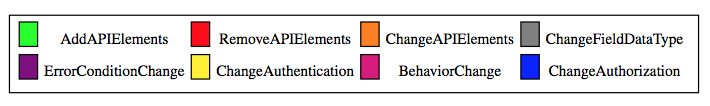
\includegraphics[keepaspectratio, width=10cm]{legend.png}
}
\end{center}
\caption{Case Study - Change Profiles for the Web APIs.}
\label{fig:proflie}
\end{figure*}


\textbf{Numbered identifiers} - Contiguous integers are used to identify new versions by Salesforce and GitHub Web APIs. Such naming scheme clearly communicates the sequence between versions but cannot be used to infer compatibility between versions.

\textbf{Timestamped identifiers} - Stripe Web API uses date as a version identifier. While timestamped versions provide the time frame of a version, they do not provide any compatibility information between versions.

\textbf{Identifiers with major and minor version numbers} - Most of the Web APIs studied use major and minor version numbers to identify a version. Facebook, Twitter, WordPress, Google Calendar, Google Maps and OpenStreetMap follow this approach. However, an explanation of the major and minor version numbers aren't provided and cannot be used to infer compatibility information.

Also, web APIs often evolve with breaking changes without issuing a new version identifier. For example, Facebook, Google Calendar and GitHub APIs often receive breaking changes without using a new version identifier.



\subsubsection{Upgrade Mode} % (fold)

From our case studies, we found the Web APIs followed several different approaches to versioning.

\textbf{Single Version} - Web APIs that force the API clients to migrate either because only one version is available or deprecated older versions will be removed. These include Facebook REST API (90 days), Twitter REST API (no specific time frame), Github API (no specific time frame), OpenStreetMap API (no specific time frame), Google Calendar (6 months), Google Maps (no specific time frame).

\textbf{Multiple Versions} - Multiple versions of the Web API are supported for longer duration. These include Wordpress REST API, Salesforce API, Stripe API.

Both of these categories, single and multiple available versions, have their advantages and disadvantages. Forcing API clients to use a single stable version makes it easy to maintain the Web APIs at the expense of scheduling flexibility for API users. These APIs keep a deprecated version for a limited period of time to provide a buffer time for the API users. For example, Google Calendar API is supporting its deprecated version for 6 months.

Maintaining multiple versions of the Web APIs provide more scheduling flexibility to the API clients but requires more effort from the API publisher. As a result, not all the older versions are maintained. When API clients lag far behind the latest version, migrating to the latest version becomes harder. For example, here is an excerpt of a comment from a Stripe Web API client developer \footnote{\url{https://groups.google.com/a/lists.stripe.com/forum/#!searchin/api-discuss/version/api-discuss/x8TM-yHnhYQ/y9JJKytSiUAJ}}:

\small
``...I just learned that we're about 14 versions behind and would like to work on upgrading but there are lots of breaking changes...''
\normalsize

While both the forced and on demand modes are found in practice, future work needs to be carried out to compare and contrast the benefits of these modes in greater detail.



\subsubsection{Change Profiles}
The Web APIs evolve at different frequencies as well as the actual change that takes place during their evolution varies from one API to another. Fig. \ref{fig:proflie} shows an aggregated view of the count of different categories of changes observed for different Web APIs based on the aforementioned coding scheme.

%
%
%\begin{figure*}[!htp]
%\begin{subfigure}[b]{\textwidth}
%\def\dataSourceFileName{facebookx.dat}
%\begin{tikzpicture}[show background rectangle,tight background]
%  \begin{axis}[
%    ybar stacked,
%    bar width=5pt,
%    %title=Facebook API Changes (11 Releases),
%    date coordinates in=x,
%    xticklabel = \year-\month,
%    xtick = {2013-01-09, 2013-04-01, 2013-07-01, 2013-10-01, 2014-01-01, 2014-04-01, 2014-08-01, 2014-07-02},
%    %xlabel={Timeline},
%    xlabel style={font=\small},
%    ylabel style={font=\small},
%    ylabel={No. of Changes},
%    xticklabel style= {rotate=90,anchor=near xticklabel,font=\tiny},
%    enlarge x limits=false,
%    height=0.20\textheight,
%    %width=\linewidth,
%    legend style={legend pos=north west,font=\tiny, legend columns=4},
%    legend to name=legend
%    ]
%    % \begin{tikzpicture}
%   \begin{axis}[
%     title=\dataSourceName\ API Changes,
%     date coordinates in=x,
%     stack plots=y,
%     area style,
%     xtick = data,
%     xlabel={Release Dates},
%     ylabel={No. of Changes},
%     xticklabel style= {rotate=90,anchor=near xticklabel,font=\tiny},
%     enlarge x limits=false,
%     height=0.25\textheight,
%     width=0.9\linewidth,
%     legend style={legend pos=north west,font=\tiny, legend columns=2}
%     ]
    \addplot[fill=green] table[x=Date, y=AddAPIElements]{plotdata/\dataSourceFileName}
    \closedcycle;
    \addplot[fill=red] table[x=Date, y=RemoveAPIElements]{plotdata/\dataSourceFileName}
    \closedcycle;
    \addplot[fill=orange] table[x=Date, y=ChangeAPIElements]{plotdata/\dataSourceFileName}
    \closedcycle;
    \addplot[fill=gray] table[x=Date, y=ChangeFieldDataType]{plotdata/\dataSourceFileName}
    \closedcycle;
    \addplot[fill=violet] table[x=Date, y=ErrorConditionChange]{plotdata/\dataSourceFileName}
    \closedcycle;
    \addplot[fill=yellow] table[x=Date, y=ChangeAuthentication]{plotdata/\dataSourceFileName}
    \closedcycle;
    \addplot[fill=magenta] table[x=Date, y=BehaviorChange]{plotdata/\dataSourceFileName}
    \closedcycle;
    \addplot[fill=blue] table[x=Date, y=ChangeAuthorization]{plotdata/\dataSourceFileName}
    \closedcycle;

    \legend{AddAPIElements, RemoveAPIElements, ChangeAPIElements,
        ChangeFieldDataType, ErrorConditionChange,
        ChangeAuthentication, BehaviorChange, ChangeAuthorization}

%   \end{axis}
% \end{tikzpicture}
%  \end{axis}
%\end{tikzpicture}
%\caption{Facebook API Changes (11 Releases)}
%\end{subfigure}
%
%\begin{subfigure}{\textwidth}
%%\caption{Stripe API Changes (30 Releases)}
%\def\dataSourceFileName{stripe.dat}
%\begin{tikzpicture}[show background rectangle,tight background]
%  \begin{axis}[
%    %title=Stripe API Changes (30 Releases),
%    date coordinates in=x,
%    ybar stacked,
%    bar width=5pt,
%    xticklabel = \year-\month,
%    xtick = {2011-09-15, 2012-01-01, 2013-01-01, 2014-01-01, 2014-10-01},
%    %xlabel={Timeline},
%    xlabel style={font=\small},
%    ylabel style={font=\small},
%    ylabel={No. of Changes},
%    xticklabel style= {rotate=90,anchor=near xticklabel,font=\tiny},
%    enlarge x limits=false,
%    height=0.20\textheight,
%    %width=\linewidth,
%    legend to name=legend
%    ]
%    % \begin{tikzpicture}
%   \begin{axis}[
%     title=\dataSourceName\ API Changes,
%     date coordinates in=x,
%     stack plots=y,
%     area style,
%     xtick = data,
%     xlabel={Release Dates},
%     ylabel={No. of Changes},
%     xticklabel style= {rotate=90,anchor=near xticklabel,font=\tiny},
%     enlarge x limits=false,
%     height=0.25\textheight,
%     width=0.9\linewidth,
%     legend style={legend pos=north west,font=\tiny, legend columns=2}
%     ]
    \addplot[fill=green] table[x=Date, y=AddAPIElements]{plotdata/\dataSourceFileName}
    \closedcycle;
    \addplot[fill=red] table[x=Date, y=RemoveAPIElements]{plotdata/\dataSourceFileName}
    \closedcycle;
    \addplot[fill=orange] table[x=Date, y=ChangeAPIElements]{plotdata/\dataSourceFileName}
    \closedcycle;
    \addplot[fill=gray] table[x=Date, y=ChangeFieldDataType]{plotdata/\dataSourceFileName}
    \closedcycle;
    \addplot[fill=violet] table[x=Date, y=ErrorConditionChange]{plotdata/\dataSourceFileName}
    \closedcycle;
    \addplot[fill=yellow] table[x=Date, y=ChangeAuthentication]{plotdata/\dataSourceFileName}
    \closedcycle;
    \addplot[fill=magenta] table[x=Date, y=BehaviorChange]{plotdata/\dataSourceFileName}
    \closedcycle;
    \addplot[fill=blue] table[x=Date, y=ChangeAuthorization]{plotdata/\dataSourceFileName}
    \closedcycle;

    \legend{AddAPIElements, RemoveAPIElements, ChangeAPIElements,
        ChangeFieldDataType, ErrorConditionChange,
        ChangeAuthentication, BehaviorChange, ChangeAuthorization}

%   \end{axis}
% \end{tikzpicture}
%  \end{axis}
%\end{tikzpicture}
%\end{subfigure}
%
%\begin{subfigure}{\textwidth}
%%\caption{WordPress REST API Changes (8 Releases)}
%\def\dataSourceFileName{wordpress.dat}
%\begin{tikzpicture}[show background rectangle,tight background]
%  \begin{axis}[
%    %title=WordPress REST API Changes (8 Releases),
%    date coordinates in=x,
%    ybar stacked,
%    bar width=5pt,
%    xticklabel = \year-\month,
%    xtick = {2013-08-07, 2013-11-01, 2014-03-01, 2014-06-26},
%    %xlabel={Timeline},
%    xlabel style={font=\small},
%    ylabel style={font=\small},
%    ylabel={No. of Changes},
%    xticklabel style= {rotate=90,anchor=near xticklabel,font=\tiny},
%    enlarge x limits=false,
%    height=0.20\textheight,
%    %width=\linewidth,
%    legend to name=legend
%    ]
%    % \begin{tikzpicture}
%   \begin{axis}[
%     title=\dataSourceName\ API Changes,
%     date coordinates in=x,
%     stack plots=y,
%     area style,
%     xtick = data,
%     xlabel={Release Dates},
%     ylabel={No. of Changes},
%     xticklabel style= {rotate=90,anchor=near xticklabel,font=\tiny},
%     enlarge x limits=false,
%     height=0.25\textheight,
%     width=0.9\linewidth,
%     legend style={legend pos=north west,font=\tiny, legend columns=2}
%     ]
    \addplot[fill=green] table[x=Date, y=AddAPIElements]{plotdata/\dataSourceFileName}
    \closedcycle;
    \addplot[fill=red] table[x=Date, y=RemoveAPIElements]{plotdata/\dataSourceFileName}
    \closedcycle;
    \addplot[fill=orange] table[x=Date, y=ChangeAPIElements]{plotdata/\dataSourceFileName}
    \closedcycle;
    \addplot[fill=gray] table[x=Date, y=ChangeFieldDataType]{plotdata/\dataSourceFileName}
    \closedcycle;
    \addplot[fill=violet] table[x=Date, y=ErrorConditionChange]{plotdata/\dataSourceFileName}
    \closedcycle;
    \addplot[fill=yellow] table[x=Date, y=ChangeAuthentication]{plotdata/\dataSourceFileName}
    \closedcycle;
    \addplot[fill=magenta] table[x=Date, y=BehaviorChange]{plotdata/\dataSourceFileName}
    \closedcycle;
    \addplot[fill=blue] table[x=Date, y=ChangeAuthorization]{plotdata/\dataSourceFileName}
    \closedcycle;

    \legend{AddAPIElements, RemoveAPIElements, ChangeAPIElements,
        ChangeFieldDataType, ErrorConditionChange,
        ChangeAuthentication, BehaviorChange, ChangeAuthorization}

%   \end{axis}
% \end{tikzpicture}
%  \end{axis}
%\end{tikzpicture}
%\end{subfigure}
%
%\begin{subfigure}{\textwidth}
%%\caption{GitHub API Changes (59 Releases)}
%\def\dataSourceFileName{github.dat}
%\begin{tikzpicture}[show background rectangle,tight background]
%  \begin{axis}[
%    %title=GitHub API Changes (59 Releases),
%    date coordinates in=x,
%    ybar stacked,
%    bar width=5pt,
%    xticklabel = \year-\month,
%    xtick = {2012-09-05, 2012-12-01, 2013-03-01, 2013-06-01, 2013-09-01, 2013-12-01, 2014-03-01, 2014-10-06},
%    %xlabel={Timeline},
%    xlabel style={font=\small},
%    ylabel style={font=\small},
%    ylabel={No. of Changes},
%    xticklabel style= {rotate=90,anchor=near xticklabel,font=\tiny},
%    enlarge x limits=false,
%    height=0.20\textheight,
%    %width=\linewidth,
%    legend to name=legend
%    ]
%    % \begin{tikzpicture}
%   \begin{axis}[
%     title=\dataSourceName\ API Changes,
%     date coordinates in=x,
%     stack plots=y,
%     area style,
%     xtick = data,
%     xlabel={Release Dates},
%     ylabel={No. of Changes},
%     xticklabel style= {rotate=90,anchor=near xticklabel,font=\tiny},
%     enlarge x limits=false,
%     height=0.25\textheight,
%     width=0.9\linewidth,
%     legend style={legend pos=north west,font=\tiny, legend columns=2}
%     ]
    \addplot[fill=green] table[x=Date, y=AddAPIElements]{plotdata/\dataSourceFileName}
    \closedcycle;
    \addplot[fill=red] table[x=Date, y=RemoveAPIElements]{plotdata/\dataSourceFileName}
    \closedcycle;
    \addplot[fill=orange] table[x=Date, y=ChangeAPIElements]{plotdata/\dataSourceFileName}
    \closedcycle;
    \addplot[fill=gray] table[x=Date, y=ChangeFieldDataType]{plotdata/\dataSourceFileName}
    \closedcycle;
    \addplot[fill=violet] table[x=Date, y=ErrorConditionChange]{plotdata/\dataSourceFileName}
    \closedcycle;
    \addplot[fill=yellow] table[x=Date, y=ChangeAuthentication]{plotdata/\dataSourceFileName}
    \closedcycle;
    \addplot[fill=magenta] table[x=Date, y=BehaviorChange]{plotdata/\dataSourceFileName}
    \closedcycle;
    \addplot[fill=blue] table[x=Date, y=ChangeAuthorization]{plotdata/\dataSourceFileName}
    \closedcycle;

    \legend{AddAPIElements, RemoveAPIElements, ChangeAPIElements,
        ChangeFieldDataType, ErrorConditionChange,
        ChangeAuthentication, BehaviorChange, ChangeAuthorization}

%   \end{axis}
% \end{tikzpicture}
%  \end{axis}
%\end{tikzpicture}
%\end{subfigure}
%
%\begin{subfigure}{\textwidth}
%%\caption{Google Maps Web API (102 Releases}
%\def\dataSourceFileName{gmap.dat}
%\begin{tikzpicture}[show background rectangle,tight background]
%  \begin{axis}[
%    %title=Google Maps Web API (102 Releases),
%    date coordinates in=x,
%    ybar stacked,
%    bar width=5pt,
%    xticklabel = \year-\month,
%    xtick = {2011-01-06, 2011-07-01, 2012-01-01, 2012-07-01, 2013-01-01, 2013-07-01, 2014-01-01, 2014-07-01, 2014-09-18},
%    %xlabel={Timeline},
%    xlabel style={font=\small},
%    ylabel style={font=\small},
%    ylabel={No. of Changes},
%    xticklabel style= {rotate=90,anchor=near xticklabel,font=\tiny},
%    enlarge x limits=false,
%    height=0.20\textheight,
%    %width=\linewidth,
%    legend to name=legend
%    ]
%    % \begin{tikzpicture}
%   \begin{axis}[
%     title=\dataSourceName\ API Changes,
%     date coordinates in=x,
%     stack plots=y,
%     area style,
%     xtick = data,
%     xlabel={Release Dates},
%     ylabel={No. of Changes},
%     xticklabel style= {rotate=90,anchor=near xticklabel,font=\tiny},
%     enlarge x limits=false,
%     height=0.25\textheight,
%     width=0.9\linewidth,
%     legend style={legend pos=north west,font=\tiny, legend columns=2}
%     ]
    \addplot[fill=green] table[x=Date, y=AddAPIElements]{plotdata/\dataSourceFileName}
    \closedcycle;
    \addplot[fill=red] table[x=Date, y=RemoveAPIElements]{plotdata/\dataSourceFileName}
    \closedcycle;
    \addplot[fill=orange] table[x=Date, y=ChangeAPIElements]{plotdata/\dataSourceFileName}
    \closedcycle;
    \addplot[fill=gray] table[x=Date, y=ChangeFieldDataType]{plotdata/\dataSourceFileName}
    \closedcycle;
    \addplot[fill=violet] table[x=Date, y=ErrorConditionChange]{plotdata/\dataSourceFileName}
    \closedcycle;
    \addplot[fill=yellow] table[x=Date, y=ChangeAuthentication]{plotdata/\dataSourceFileName}
    \closedcycle;
    \addplot[fill=magenta] table[x=Date, y=BehaviorChange]{plotdata/\dataSourceFileName}
    \closedcycle;
    \addplot[fill=blue] table[x=Date, y=ChangeAuthorization]{plotdata/\dataSourceFileName}
    \closedcycle;

    \legend{AddAPIElements, RemoveAPIElements, ChangeAPIElements,
        ChangeFieldDataType, ErrorConditionChange,
        ChangeAuthentication, BehaviorChange, ChangeAuthorization}

%   \end{axis}
% \end{tikzpicture}
%  \end{axis}
%\end{tikzpicture}
%\end{subfigure}
%
%\begin{subfigure}{\textwidth}
%%\caption{[Salesforce REST API (4 Releases)]}
%\def\dataSourceName{Salesforce Force.com and Chatter REST}
%\def\dataSourceFileName{salesforce.dat}
%\begin{tikzpicture}[show background rectangle,tight background]
%  \begin{axis}[
%    %title=Salesforce REST API (4 Releases),
%    date coordinates in=x,
%    ybar stacked,
%    bar width=5pt,
%    xticklabel = \year-\month,
%    xtick = {2013-10-04, 2014-01-01, 2014-04-01, 2014-07-01, 2014-10-18},
%    %label={Timeline},
%    xlabel style={font=\small},
%    ylabel style={font=\small},
%    ylabel={No. of Changes},
%    xticklabel style= {rotate=90,anchor=near xticklabel,font=\tiny},
%    enlarge x limits=false,
%    height=0.20\textheight,
%    %width=0.9\linewidth,
%    legend to name=legend
%    ]
%    % \begin{tikzpicture}
%   \begin{axis}[
%     title=\dataSourceName\ API Changes,
%     date coordinates in=x,
%     stack plots=y,
%     area style,
%     xtick = data,
%     xlabel={Release Dates},
%     ylabel={No. of Changes},
%     xticklabel style= {rotate=90,anchor=near xticklabel,font=\tiny},
%     enlarge x limits=false,
%     height=0.25\textheight,
%     width=0.9\linewidth,
%     legend style={legend pos=north west,font=\tiny, legend columns=2}
%     ]
    \addplot[fill=green] table[x=Date, y=AddAPIElements]{plotdata/\dataSourceFileName}
    \closedcycle;
    \addplot[fill=red] table[x=Date, y=RemoveAPIElements]{plotdata/\dataSourceFileName}
    \closedcycle;
    \addplot[fill=orange] table[x=Date, y=ChangeAPIElements]{plotdata/\dataSourceFileName}
    \closedcycle;
    \addplot[fill=gray] table[x=Date, y=ChangeFieldDataType]{plotdata/\dataSourceFileName}
    \closedcycle;
    \addplot[fill=violet] table[x=Date, y=ErrorConditionChange]{plotdata/\dataSourceFileName}
    \closedcycle;
    \addplot[fill=yellow] table[x=Date, y=ChangeAuthentication]{plotdata/\dataSourceFileName}
    \closedcycle;
    \addplot[fill=magenta] table[x=Date, y=BehaviorChange]{plotdata/\dataSourceFileName}
    \closedcycle;
    \addplot[fill=blue] table[x=Date, y=ChangeAuthorization]{plotdata/\dataSourceFileName}
    \closedcycle;

    \legend{AddAPIElements, RemoveAPIElements, ChangeAPIElements,
        ChangeFieldDataType, ErrorConditionChange,
        ChangeAuthentication, BehaviorChange, ChangeAuthorization}

%   \end{axis}
% \end{tikzpicture}
%  \end{axis}
%\end{tikzpicture}
%\end{subfigure}
%
%\begin{subfigure}{\textwidth}
%\ref{legend}
%\end{subfigure}
%
%\caption{Case Study - Change Profiles for the Web APIs.}
%\end{figure*}
%

%%%%%%%%%%%%%%%%%%
%
%x.dat}
%\begin{tikzpicture}[show background rectangle,tight background]
%  \begin{axis}[
%    ybar stacked,
%    bar width=5pt,
%    title=Facebook API Changes (11 Releases),
%    date coordinates in=x,
%    xticklabel = \year-\month,
%    xtick = {2013-01-09, 2013-04-01, 2013-07-01, 2013-10-01, 2014-01-01, 2014-04-01, 2014-08-01, 2014-07-02},
%    xlabel={Timeline},
%    xlabel style={font=\small},
%    ylabel style={font=\small},
%    ylabel={No. of Changes},
%    xticklabel style= {rotate=90,anchor=near xticklabel,font=\tiny},
%    enlarge x limits=false,
%    height=0.20\textheight,
%    width=\linewidth,
%    legend style={legend pos=north west,font=\tiny, legend columns=4},
%    legend to name=legend
%    ]
%    % \begin{tikzpicture}
%   \begin{axis}[
%     title=\dataSourceName\ API Changes,
%     date coordinates in=x,
%     stack plots=y,
%     area style,
%     xtick = data,
%     xlabel={Release Dates},
%     ylabel={No. of Changes},
%     xticklabel style= {rotate=90,anchor=near xticklabel,font=\tiny},
%     enlarge x limits=false,
%     height=0.25\textheight,
%     width=0.9\linewidth,
%     legend style={legend pos=north west,font=\tiny, legend columns=2}
%     ]
    \addplot[fill=green] table[x=Date, y=AddAPIElements]{plotdata/\dataSourceFileName}
    \closedcycle;
    \addplot[fill=red] table[x=Date, y=RemoveAPIElements]{plotdata/\dataSourceFileName}
    \closedcycle;
    \addplot[fill=orange] table[x=Date, y=ChangeAPIElements]{plotdata/\dataSourceFileName}
    \closedcycle;
    \addplot[fill=gray] table[x=Date, y=ChangeFieldDataType]{plotdata/\dataSourceFileName}
    \closedcycle;
    \addplot[fill=violet] table[x=Date, y=ErrorConditionChange]{plotdata/\dataSourceFileName}
    \closedcycle;
    \addplot[fill=yellow] table[x=Date, y=ChangeAuthentication]{plotdata/\dataSourceFileName}
    \closedcycle;
    \addplot[fill=magenta] table[x=Date, y=BehaviorChange]{plotdata/\dataSourceFileName}
    \closedcycle;
    \addplot[fill=blue] table[x=Date, y=ChangeAuthorization]{plotdata/\dataSourceFileName}
    \closedcycle;

    \legend{AddAPIElements, RemoveAPIElements, ChangeAPIElements,
        ChangeFieldDataType, ErrorConditionChange,
        ChangeAuthentication, BehaviorChange, ChangeAuthorization}

%   \end{axis}
% \end{tikzpicture}
%  \end{axis}
%\end{tikzpicture}
%
%
%\ref{legend}
%
%\def\dataSourceFileName{stripe.dat}
%\begin{tikzpicture}[show background rectangle,tight background]
%  \begin{axis}[
%    title=Stripe API Changes (30 Releases),
%    date coordinates in=x,
%    ybar stacked,
%    bar width=5pt,
%    xticklabel = \year-\month,
%    xtick = {2011-09-15, 2012-01-01, 2013-01-01, 2014-01-01, 2014-10-01},
%    xlabel={Timeline},
%    xlabel style={font=\small},
%    ylabel style={font=\small},
%    ylabel={No. of Changes},
%    xticklabel style= {rotate=90,anchor=near xticklabel,font=\tiny},
%    enlarge x limits=false,
%    height=0.20\textheight,
%    width=\linewidth,
%    legend to name=legend
%    ]
%    % \begin{tikzpicture}
%   \begin{axis}[
%     title=\dataSourceName\ API Changes,
%     date coordinates in=x,
%     stack plots=y,
%     area style,
%     xtick = data,
%     xlabel={Release Dates},
%     ylabel={No. of Changes},
%     xticklabel style= {rotate=90,anchor=near xticklabel,font=\tiny},
%     enlarge x limits=false,
%     height=0.25\textheight,
%     width=0.9\linewidth,
%     legend style={legend pos=north west,font=\tiny, legend columns=2}
%     ]
    \addplot[fill=green] table[x=Date, y=AddAPIElements]{plotdata/\dataSourceFileName}
    \closedcycle;
    \addplot[fill=red] table[x=Date, y=RemoveAPIElements]{plotdata/\dataSourceFileName}
    \closedcycle;
    \addplot[fill=orange] table[x=Date, y=ChangeAPIElements]{plotdata/\dataSourceFileName}
    \closedcycle;
    \addplot[fill=gray] table[x=Date, y=ChangeFieldDataType]{plotdata/\dataSourceFileName}
    \closedcycle;
    \addplot[fill=violet] table[x=Date, y=ErrorConditionChange]{plotdata/\dataSourceFileName}
    \closedcycle;
    \addplot[fill=yellow] table[x=Date, y=ChangeAuthentication]{plotdata/\dataSourceFileName}
    \closedcycle;
    \addplot[fill=magenta] table[x=Date, y=BehaviorChange]{plotdata/\dataSourceFileName}
    \closedcycle;
    \addplot[fill=blue] table[x=Date, y=ChangeAuthorization]{plotdata/\dataSourceFileName}
    \closedcycle;

    \legend{AddAPIElements, RemoveAPIElements, ChangeAPIElements,
        ChangeFieldDataType, ErrorConditionChange,
        ChangeAuthentication, BehaviorChange, ChangeAuthorization}

%   \end{axis}
% \end{tikzpicture}
%  \end{axis}
%\end{tikzpicture}
%
%
%\def\dataSourceFileName{wordpress.dat}
%\begin{tikzpicture}[show background rectangle,tight background]
%  \begin{axis}[
%    title=WorPress REST API Changes (8 Releases),
%    date coordinates in=x,
%    ybar stacked,
%    bar width=5pt,
%    xticklabel = \year-\month,
%    xtick = {2013-08-07, 2013-11-01, 2014-03-01, 2014-06-26},
%    xlabel={Timeline},
%    xlabel style={font=\small},
%    ylabel style={font=\small},
%    ylabel={No. of Changes},
%    xticklabel style= {rotate=90,anchor=near xticklabel,font=\tiny},
%    enlarge x limits=false,
%    height=0.20\textheight,
%    width=\linewidth,
%    legend to name=legend
%    ]
%    % \begin{tikzpicture}
%   \begin{axis}[
%     title=\dataSourceName\ API Changes,
%     date coordinates in=x,
%     stack plots=y,
%     area style,
%     xtick = data,
%     xlabel={Release Dates},
%     ylabel={No. of Changes},
%     xticklabel style= {rotate=90,anchor=near xticklabel,font=\tiny},
%     enlarge x limits=false,
%     height=0.25\textheight,
%     width=0.9\linewidth,
%     legend style={legend pos=north west,font=\tiny, legend columns=2}
%     ]
    \addplot[fill=green] table[x=Date, y=AddAPIElements]{plotdata/\dataSourceFileName}
    \closedcycle;
    \addplot[fill=red] table[x=Date, y=RemoveAPIElements]{plotdata/\dataSourceFileName}
    \closedcycle;
    \addplot[fill=orange] table[x=Date, y=ChangeAPIElements]{plotdata/\dataSourceFileName}
    \closedcycle;
    \addplot[fill=gray] table[x=Date, y=ChangeFieldDataType]{plotdata/\dataSourceFileName}
    \closedcycle;
    \addplot[fill=violet] table[x=Date, y=ErrorConditionChange]{plotdata/\dataSourceFileName}
    \closedcycle;
    \addplot[fill=yellow] table[x=Date, y=ChangeAuthentication]{plotdata/\dataSourceFileName}
    \closedcycle;
    \addplot[fill=magenta] table[x=Date, y=BehaviorChange]{plotdata/\dataSourceFileName}
    \closedcycle;
    \addplot[fill=blue] table[x=Date, y=ChangeAuthorization]{plotdata/\dataSourceFileName}
    \closedcycle;

    \legend{AddAPIElements, RemoveAPIElements, ChangeAPIElements,
        ChangeFieldDataType, ErrorConditionChange,
        ChangeAuthentication, BehaviorChange, ChangeAuthorization}

%   \end{axis}
% \end{tikzpicture}
%  \end{axis}
%\end{tikzpicture}
%
%
%\def\dataSourceFileName{github.dat}
%\begin{tikzpicture}[show background rectangle,tight background]
%  \begin{axis}[
%    title=GitHub API Changes (59 Releases),
%    date coordinates in=x,
%    ybar stacked,
%    bar width=5pt,
%    xticklabel = \year-\month,
%    xtick = {2012-09-05, 2012-12-01, 2013-03-01, 2013-06-01, 2013-09-01, 2013-12-01, 2014-03-01, 2014-10-06},
%    xlabel={Timeline},
%    xlabel style={font=\small},
%    ylabel style={font=\small},
%    ylabel={No. of Changes},
%    xticklabel style= {rotate=90,anchor=near xticklabel,font=\tiny},
%    enlarge x limits=false,
%    height=0.20\textheight,
%    width=\linewidth,
%    legend to name=legend
%    ]
%    % \begin{tikzpicture}
%   \begin{axis}[
%     title=\dataSourceName\ API Changes,
%     date coordinates in=x,
%     stack plots=y,
%     area style,
%     xtick = data,
%     xlabel={Release Dates},
%     ylabel={No. of Changes},
%     xticklabel style= {rotate=90,anchor=near xticklabel,font=\tiny},
%     enlarge x limits=false,
%     height=0.25\textheight,
%     width=0.9\linewidth,
%     legend style={legend pos=north west,font=\tiny, legend columns=2}
%     ]
    \addplot[fill=green] table[x=Date, y=AddAPIElements]{plotdata/\dataSourceFileName}
    \closedcycle;
    \addplot[fill=red] table[x=Date, y=RemoveAPIElements]{plotdata/\dataSourceFileName}
    \closedcycle;
    \addplot[fill=orange] table[x=Date, y=ChangeAPIElements]{plotdata/\dataSourceFileName}
    \closedcycle;
    \addplot[fill=gray] table[x=Date, y=ChangeFieldDataType]{plotdata/\dataSourceFileName}
    \closedcycle;
    \addplot[fill=violet] table[x=Date, y=ErrorConditionChange]{plotdata/\dataSourceFileName}
    \closedcycle;
    \addplot[fill=yellow] table[x=Date, y=ChangeAuthentication]{plotdata/\dataSourceFileName}
    \closedcycle;
    \addplot[fill=magenta] table[x=Date, y=BehaviorChange]{plotdata/\dataSourceFileName}
    \closedcycle;
    \addplot[fill=blue] table[x=Date, y=ChangeAuthorization]{plotdata/\dataSourceFileName}
    \closedcycle;

    \legend{AddAPIElements, RemoveAPIElements, ChangeAPIElements,
        ChangeFieldDataType, ErrorConditionChange,
        ChangeAuthentication, BehaviorChange, ChangeAuthorization}

%   \end{axis}
% \end{tikzpicture}
%  \end{axis}
%\end{tikzpicture}
%
%\def\dataSourceFileName{gmap.dat}
%\begin{tikzpicture}[show background rectangle,tight background]
%  \begin{axis}[
%    title=Google Maps Web API (102 Releases),
%    date coordinates in=x,
%    ybar stacked,
%    bar width=5pt,
%    xticklabel = \year-\month,
%    xtick = {2011-01-06, 2011-07-01, 2012-01-01, 2012-07-01, 2013-01-01, 2013-07-01, 2014-01-01, 2014-07-01, 2014-09-18},
%    xlabel={Timeline},
%    xlabel style={font=\small},
%    ylabel style={font=\small},
%    ylabel={No. of Changes},
%    xticklabel style= {rotate=90,anchor=near xticklabel,font=\tiny},
%    enlarge x limits=false,
%    height=0.20\textheight,
%    width=\linewidth,
%    legend to name=legend
%    ]
%    % \begin{tikzpicture}
%   \begin{axis}[
%     title=\dataSourceName\ API Changes,
%     date coordinates in=x,
%     stack plots=y,
%     area style,
%     xtick = data,
%     xlabel={Release Dates},
%     ylabel={No. of Changes},
%     xticklabel style= {rotate=90,anchor=near xticklabel,font=\tiny},
%     enlarge x limits=false,
%     height=0.25\textheight,
%     width=0.9\linewidth,
%     legend style={legend pos=north west,font=\tiny, legend columns=2}
%     ]
    \addplot[fill=green] table[x=Date, y=AddAPIElements]{plotdata/\dataSourceFileName}
    \closedcycle;
    \addplot[fill=red] table[x=Date, y=RemoveAPIElements]{plotdata/\dataSourceFileName}
    \closedcycle;
    \addplot[fill=orange] table[x=Date, y=ChangeAPIElements]{plotdata/\dataSourceFileName}
    \closedcycle;
    \addplot[fill=gray] table[x=Date, y=ChangeFieldDataType]{plotdata/\dataSourceFileName}
    \closedcycle;
    \addplot[fill=violet] table[x=Date, y=ErrorConditionChange]{plotdata/\dataSourceFileName}
    \closedcycle;
    \addplot[fill=yellow] table[x=Date, y=ChangeAuthentication]{plotdata/\dataSourceFileName}
    \closedcycle;
    \addplot[fill=magenta] table[x=Date, y=BehaviorChange]{plotdata/\dataSourceFileName}
    \closedcycle;
    \addplot[fill=blue] table[x=Date, y=ChangeAuthorization]{plotdata/\dataSourceFileName}
    \closedcycle;

    \legend{AddAPIElements, RemoveAPIElements, ChangeAPIElements,
        ChangeFieldDataType, ErrorConditionChange,
        ChangeAuthentication, BehaviorChange, ChangeAuthorization}

%   \end{axis}
% \end{tikzpicture}
%  \end{axis}
%\end{tikzpicture}
%
%\def\dataSourceName{Salesforce Force.com and Chatter REST}
%\def\dataSourceFileName{salesforce.dat}
%\begin{tikzpicture}[show background rectangle,tight background]
%  \begin{axis}[
%    title=Salesforce REST API (4 Releases),
%    date coordinates in=x,
%    ybar stacked,
%    bar width=5pt,
%    xticklabel = \year-\month,
%    xtick = {2013-10-04, 2014-01-01, 2014-04-01, 2014-07-01, 2014-10-18},
%    xlabel={Timeline},
%    xlabel style={font=\small},
%    ylabel style={font=\small},
%    ylabel={No. of Changes},
%    xticklabel style= {rotate=90,anchor=near xticklabel,font=\tiny},
%    enlarge x limits=false,
%    height=0.20\textheight,
%    width=0.9\linewidth,
%    legend to name=legend
%    ]
%    % \begin{tikzpicture}
%   \begin{axis}[
%     title=\dataSourceName\ API Changes,
%     date coordinates in=x,
%     stack plots=y,
%     area style,
%     xtick = data,
%     xlabel={Release Dates},
%     ylabel={No. of Changes},
%     xticklabel style= {rotate=90,anchor=near xticklabel,font=\tiny},
%     enlarge x limits=false,
%     height=0.25\textheight,
%     width=0.9\linewidth,
%     legend style={legend pos=north west,font=\tiny, legend columns=2}
%     ]
    \addplot[fill=green] table[x=Date, y=AddAPIElements]{plotdata/\dataSourceFileName}
    \closedcycle;
    \addplot[fill=red] table[x=Date, y=RemoveAPIElements]{plotdata/\dataSourceFileName}
    \closedcycle;
    \addplot[fill=orange] table[x=Date, y=ChangeAPIElements]{plotdata/\dataSourceFileName}
    \closedcycle;
    \addplot[fill=gray] table[x=Date, y=ChangeFieldDataType]{plotdata/\dataSourceFileName}
    \closedcycle;
    \addplot[fill=violet] table[x=Date, y=ErrorConditionChange]{plotdata/\dataSourceFileName}
    \closedcycle;
    \addplot[fill=yellow] table[x=Date, y=ChangeAuthentication]{plotdata/\dataSourceFileName}
    \closedcycle;
    \addplot[fill=magenta] table[x=Date, y=BehaviorChange]{plotdata/\dataSourceFileName}
    \closedcycle;
    \addplot[fill=blue] table[x=Date, y=ChangeAuthorization]{plotdata/\dataSourceFileName}
    \closedcycle;

    \legend{AddAPIElements, RemoveAPIElements, ChangeAPIElements,
        ChangeFieldDataType, ErrorConditionChange,
        ChangeAuthentication, BehaviorChange, ChangeAuthorization}

%   \end{axis}
% \end{tikzpicture}
%  \end{axis}
%\end{tikzpicture}

The APIs here show very different change trajectories. Facebook API shows an alternating pattern of smaller and larger number of changes between subsequent versions, and each release consists of multiple categories of changes. On the other hand, Stripe and GitHub API changes are more frequent, but on the majority of the releases only include a single category of change. WordPress REST API releases contain multiple categories of changes, but shows only a single API element removal for the studied period. GoogleMaps API changes are also very frequent, dominated by AddAPIElement and BehaviorChange categories in a way that once new API elements are introduced, the subsequent releases primarily focus on bug fixes. The GoogleMaps API shows signs of stability with time. The Salesforce API changelog shows a different picture. Unlike the other APIs studied, Salesforce API evolves quarterly and involves a larger number of API elements with each release. We observed most Web API releases broke backward compatibility as shown by the presence of colors in addition to the green areas on the charts. We consider API changes to be backward compatible when changes are limited to only AddAPIElements category.

Google Calendar API, not shown in a chart, changed the format of all API request and response data from a custom XML to JSON in a single release, effectively forcing all its users to upgrade with a deprecation policy of one year. A plot for the Twitter and OpenStreetMap APIs could not be produced since changelogs for these APIs were no longer available.

These change profiles have little similarity, implying the fact that a common solution to solve their evolution related challenges may not work. Future research on Web API evolution needs to consider these variation of change profiles to find effective solutions for the case in hand.

\subsubsection{Implementation} % (fold)
\label{ssub:implementation}

In our case studies, we included two open-source Web APIs, WordPress and OpenStreetMap, because it gave us access to  their source code to study how versioning is actually implemented. Wordpress REST API is developed as a plugin for Wordpress. As a result, a new version of the Web API is released with a new version of the plugin and it all API clients are affected when a new version is deployed. The source code for OpenStreetMap.org Web API shows the use of configuration files for API Versioning. We found its implementation only allows for a single API version.

To summarize the change profiles, version identifiers and implementation of evolving Web API versions, we observed little convergence and a lack of any common scheme that was followed by the studied Web APIs.

\subsection{RQ2 Documentation} % (fold)
\label{sub:documentation}
Web API documentation is used by API users as the primary source of information for system integration. We analyzed the API reference documentation to understand the contents and the presentation style of their documentation. The documentation is commonly comprised of the following:

\textbf{Web API access information} - Web API documentation includes information about the URL where the API can be reached. The studied APIs used one of the URL, HTTP headers, or a user interface to identify specific API versions.

\textbf{Authentication} - Web API documentation includes information about authentication for their API clients. This is also used to implement client specific rules, such as rate limits and time zones.

\textbf{API Interface definition} - The interface definition is a major part of the Web API documentation where each API element is described with a general overview  and related business rules.

\textbf{Example usage} - Examples that describe different use cases of the Web APIs are also commonly found in the documentation. The examples contain the data and HTTP headers for sample requests and the corresponding API responses.

Some of the studied Web APIs also provide live web browser based API explorers, where API users can make API calls without needing to write any code. However, the studied Web APIs that offered Live API Explorer only did so for the latest API versions.

Web API documentation needs to include additional information compared to local APIs since HTTP is used for communication. As an API evolves lack of documentation for older API versions causes difficulties with the upgrade process as found in the following comment from a Stripe API user\footnote{\url{https://groups.google.com/a/lists.stripe.com/forum/#!searchin/api-discuss/version/api-discuss/li4PyVcweiw/NT9SFTtF-vQJ}}

\small
\begin{quotation}
 ``Does the full API documentation only reflect the current version of the
  API?  Is there a way to access the API docs for outdated versions? ...That would be very helpful. When you are trying to upgrade from one version to another it's impossible to know the implementation differences. We are currently about 4 API versions behind and are stuck behind a version that causes a significant amount of work on our end to support. I'd like to be able to upgrade incrementally through each version.''
\end{quotation}
\normalsize

We also investigated how the API documentation is generated. We found that, Web API documents are manually generated and updated, unlike the documentation for local APIs which are are typically auto-generated. For WordPress and OpenStreetMap, this is apparent from their source code, as we found the use of manually edited wiki and Markdown files to generate the documentation\footnote{\url{http://en.wikipedia.org/wiki/Markdown}}.

In our case studies, we found one example of self-documenting Web API as discussed by Laskey \cite{laskey2008considerations}. The Salesforce Web API has API endpoints that describe all available versions of the API that can be used to programmatically determine the changes between versions.

To summarize, we found that Web API documents are manually generated and widely vary in terms of both their contents and presentation formats.

\subsection{RQ3 Communication} % (fold)
\label{sub:communication}

Communicating updates and changelogs is an important activity for evolving Web APIs. The communication channels used by the studied Web APIs is categorized as follows:


  \textbf{API home page} - Web APIs announce the API changes in their home pages. In practice, the announcements include partial change log with the key changes that are made in a release. These announcements are unstructured text and do not follow any standard format even for the same API.

  \textbf{API response} - Some Web APIs use custom HTTP headers to indicate when a call is made to a deprecated version. For example, Wordpress REST API sends the X-WP-DeprecatedFunction header in response to API calls made to deprecated endpoints.

  \textbf{Email} - Facebook sends customized email alerts to its API clients based on their usage of the API, similar to the idea as presented by Zou et al. \cite{le2008synchronizing}. API calls are recorded to determine if a change has an impact on users. The granularity of the change tracking often results into false-positives, as found in this comment by a Facebook API user \footnote{\url{http://stackoverflow.com/questions/16270446/updating-app-for-breaking-change-non-threaded-comments}}:

\small
\begin{quotation}
...I have received the same notification for one of my apps. My app definitely does not read or create comments on Facebook posts or objects ... Thus Facebook's message is not relevant to every app they send it to.
The change should only affect apps which read or publish comments.
\end{quotation}
\normalsize

  \textbf{Newsfeed} - To keep up-to-date with API changes, the Web API clients are requested to subscribe to newsfeed, typically delivered via mailing lists and Twitter feeds. User feedback is also collected on these platforms. For example, at the time of writing this paper there were 13,239 questions tagged against google-maps-api-3\footnote{\url{https://stackoverflow.com/questions/tagged/google-maps-api-313.239}}.


To summarize, we found both formal and informal channels are used to communicate Web API changes. Most messages are primarily driven by manually edited unstructured text.
% subsection communication (end)

\section{Discussion} % (fold)
\label{sec:discussion}
Our case study findings such as a lack of standard approaches to deal with Web API versioning, documentation and change communication confirms the findings from previous case studies. In addition to the Web API change patterns identified by previous case studies, we have identified six new change patterns: 1) move API elements, 2) rename API elements, 3) behavior change, 4) post condition change, 5) HTTP header change, and 6) error condition change. When creating API changelog and developing related tool support, these new change patterns can be used to communicate the changes using a shared vocabulary. In addition to these new change patterns, from our case study we have compiled a list of recommendations and identified new research problems related to RQ1-3 as discussed in the following paragraphs.

\textbf{RQ1 Versioning} - From our case study, we found that when a new version is released for a Web API, the version identifiers provide little information about backward compatibility and the impact of the new version on existing API users. As a result, the API users are left to follow the free-form newsfeeds to understand the impact for each new API version. To improve this situation, for practitioners, we recommend using Semantic Versioning. Semantic Versioning is a naming technique for versioning software so that it is possible to infer if two versions are backward compatible simply by interpreting the version identifiers\footnote{\url{http://semver.org/}}. Future research can be carried out to automatically generate a Semantic Versioning identifier based on the compatibility between versions.

Our change profiles show that Web APIs often evolve as fast as several times a month and forces API clients to upgrade. Also, releases often combine both bug fixes and other breaking changes, forcing the API users to adapt even though they only need the fixes.  For practitioners, we recommend that bug fixes and breaking changes be released under separate versions to provide more flexibility to the API clients. Future research needs to focus on finding strategies for evolving Web APIs so that bug fixes and other changes can be easily delivered in separate versions and multiple versions can be made available at the same time.

\textbf{RQ2 Documentation} - We observed a that largely manual process is used for generating API documentation for most RESTful APIs. Manually generating and maintaining such documentation is expensive and error-prone. From our analysis, we showed that even when Web APIs are  versioned, documentation for older versions is not always available, and the difference between two versions of a Web API cannot be easily derived from their manually edited API references. We also found that the changelogs and API references are two disconnected documents even though a user needs to read both documents while upgrading. For practitioners, we recommend releasing Web API documentation for each available version that is cross-linked with the changelog. Future research on tool development can be aimed to support automated, version-aware documentation needs of evolving Web APIs.

Live Web API explorers are used by API users to try the APIs with little effort. However, there is a lack of reusable approach to create Live Web API explorers and bespoke implementation of the live API explorers are expensive since they need additional software development. We have seen only two of the nine studied APIs to provide a live API explorer. Moreover, we found that live Web API explorers are only offered for latest versions. Future research can focus on the implementation of a reusable, version-aware live Web API explorer for evolving Web APIs.

Self documenting Web APIs can be used to automatically determine compatibility between two versions of a Web API. We found Salesforce REST API to be the only example from our case studies that implemented self documenting Web APIs. For practitioners, we recommend providing self-documenting Web APIs. We also identify this as an opportunity for future research so that reusable tool support can be provided to create self-documenting Web APIS.

\textbf{RQ3 Communication} - For communicating API changes, we found a number of different channels that are used in practice. These channels need to be compared so that the effective channels can be used for communicating between the API developers and users.

In the change profiles we found the APIs change frequently and this requires manual effort to understand the impact of a change on a specific API user. This can be simplified by alerting users about an API change with a customized changelog. We also found that API related discussions are carried out external to the API documentation sites. API users need to search multiple disconnected information sources when API related questions arise. For practitioners, we recommend publishing a customized changelog for their Web APIs and providing discussion forums with API documentation. Previous research showed a solution based on WSDL files \cite{le2008synchronizing}. Future research is needed to solve this problem for RESTful Web APIs.

The open source Web APIs (Wordpress and OpenStreetMap) had limited documentation and change log information compared to the proprietary Web APIs. This presents an opportunity for researchers and industry practitioners to create reusable open source versioning and documentation tools for evolving Web APIs.

\textbf{Limitations} - We recognize the number of Web APIs studied to be a threat to the construct validity. Although our selection involves a diverse set of Web APIs, the findings may not be generalized for all evolving Web APIs. Our selection criteria included different industry domains, API sizes, popularity and maturity levels to minimize selection bias. The selected APIs represent only publicly available evolving Web APIs because only publicly available data is used for the case study. Future work need to be carried out to compare the applicability of our findings and related implications on privately maintained evolving Web APIs. To mitigate the interpretation bias of the coding scheme, the first two authors of this paper independently annotated randomly selected snippets of change logs from different Web APIs and reached the same conclusion indicating the replicability of the given coding scheme.

Given the state of practice we found a wide variety of ways to evolve Web APIs in terms of versioning, documentation and communication of changes and no consistent way to deal with the changes. This indicates an immature area where cost-effective solutions that are acceptable for both API developers and users are still missing - as discussed. Further research needs to be carried out to validate the usefulness of the aforementioned recommendations and solve the new research problems as identified by this case study.

\section{Conclusion}
Web API evolution poses challenges since a change may break applications that are developed by different teams and organizations. We presented a case study of Web API evolution focusing on the challenges involved with versioning, documentation and communication of API changes. Recommendations for practitioners from our analysis include the use of semantic versioning, separate releases for bug fixes and new features, auto generated API documentation cross-linked with changelogs and providing live API explorers. A list of open research problems are discussed related to Web API evolution that we want to solve in our future work.

\bibliographystyle{./IEEEtran}
\bibliography{IEEEabrv,references}

\end{document}


